\documentclass[14pt]{extarticle}
%Some packages I commonly use.
\usepackage[english]{babel}
\usepackage{graphicx}
\usepackage{framed}
\usepackage[normalem]{ulem}
\usepackage{amsmath}
\usepackage{amsthm}
\usepackage{amssymb}
\usepackage{amsfonts}
\usepackage{enumerate}
\usepackage[utf8]{inputenc}
\usepackage[top=1 in,bottom=1in, left=1 in, right=1 in]{geometry}
\usepackage{multirow}
\usepackage{colortbl}
\definecolor{kugray5}{RGB}{224,224,224}
 

%A bunch of definitions that make my life easier
\newcommand{\matlab}{{\sc Matlab} }
\newcommand{\cvec}[1]{{\mathbf #1}}
\newcommand{\rvec}[1]{\vec{\mathbf #1}}
\newcommand{\ihat}{\hat{\textbf{\i}}}
\newcommand{\jhat}{\hat{\textbf{\j}}}
\newcommand{\khat}{\hat{\textbf{k}}}
\newcommand{\minor}{{\rm minor}}
\newcommand{\trace}{{\rm trace}}
\newcommand{\spn}{{\rm Span}}
\newcommand{\rem}{{\rm rem}}
\newcommand{\ran}{{\rm range}}
\newcommand{\range}{{\rm range}}
\newcommand{\mdiv}{{\rm div}}
\newcommand{\proj}{{\rm proj}}
\newcommand{\R}{\mathbb{R}}
\newcommand{\N}{\mathbb{N}}
\newcommand{\Q}{\mathbb{Q}}
\newcommand{\Z}{\mathbb{Z}}
\newcommand{\<}{\langle}
\renewcommand{\>}{\rangle}
\renewcommand{\emptyset}{\varnothing}
\newcommand{\attn}[1]{\textbf{#1}}
\theoremstyle{definition}
\newtheorem{theorem}{Theorem}
\newtheorem{corollary}{Corollary}
\newtheorem*{definition}{Definition}
\newtheorem*{example}{Example}
\newtheorem*{note}{Note}
\newtheorem{exercise}{Exercise}
\newcommand{\bproof}{\bigskip {\bf Proof. }}
\newcommand{\eproof}{\hfill\qedsymbol}
\newcommand{\Disp}{\displaystyle}
\newcommand{\qe}{\hfill\(\bigtriangledown\)}
\setlength{\columnseprule}{1 pt}
\usepackage{graphicx}
\graphicspath{ {images/} }
\usepackage[nottoc]{tocbibind}



% \title{Handwritten Text Recognition}
% 
\includegraphics[]{cinnamon.png}
% \author{Bigkizd}
% \date{Feb 2019}

\begin{document}
\begin{titlepage}
\begin{center}
{\LARGE PHASE 2 RESEARCH PROPOSAL}\\[1.5cm]
\linespread{1.2}\huge {\bfseries Handwritten Text Recognition}\\[1.5cm]
\linespread{1}

\includegraphics[width=17cm]{cinnamon.png}\\[1cm]
{\Large Bigkizd}\\[1cm]
% {\large \emph{Supervisor:} Supervisor's Name}\\[1cm] % if applicable
% \large A report submitted in partial fulfilment of the requirements\\ for the degree of ???? in Computer Science\\[0.3cm] 
% \textit{in the}\\[0.3cm]
% Department of Computer Science\\[2cm]

\today
\end{center}

\end{titlepage}

\section{Introduction}
The handwriten text recognition is a challenging problem and has been attended by numerous researchers. The accuracy belong to the style of write and the collected data. Most of the traditional offline handwritten Janpanese/Chinese text recognizers perform segmentation of text image into characters before individually recognizing each character and integrating linguistic and geometric contexts. With the growth of Deep Learning and Connectionist Temporal Classification algorithm(CTC), I would like to build an end-to-end text recognition model for learning to recognize text from a whole handwritten line text. 
\section{Problem Statement}
\begin{itemize}
    \item Input: an image about a line of text 
    \item Output: extracted text from input image
\end{itemize}
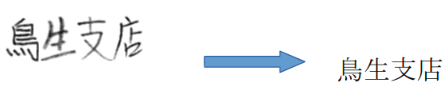
\includegraphics[width=170mm,scale=0.7]{statement.png}
\section{Related word}
 I have researched two approaches about handwriting optical character recognition. The first, segment and decode, segment image into character based image, then using classification for each character segment previous.I not recommend this method, because when segmentation error leads to ouput error.  The second, non-segmentation, it includes hidden Markov models(HMMs), time-decay neural networks(TDNN), and recurrent neural networks(RNN) combination of Convolutional Neural Networks and Recurrent Neural Networks(CRNN) with techniques specific case attention in deep learning\cite{crnn}. 

I have follow a model CRNN or CRNN with attention macharism. It is good baseline model to follow because:  
\begin{itemize}
    \item No need detector or cropping technique to find a character like segmentation and decode. 
    \item Sequence data of arbiitrary length can be processed because of LSTM which is free in size of input and output sequence. 
    \item It is model end to end learning algorithm. 
\end{itemize}
\section{Our Approach}
\subsection{Exploratory Data Analysis}
\subsubsection{Data Collection}
Current, we have synthesis data from our company. After, I start collection data by the training(80\%) and testing(20\%) dataset into Pytorch.
Description Dataset: Current, we have 402463 image.
\subsubsection{Data Preprocessing}
I have histogram of each input variable to get an idea of distribution: \newline
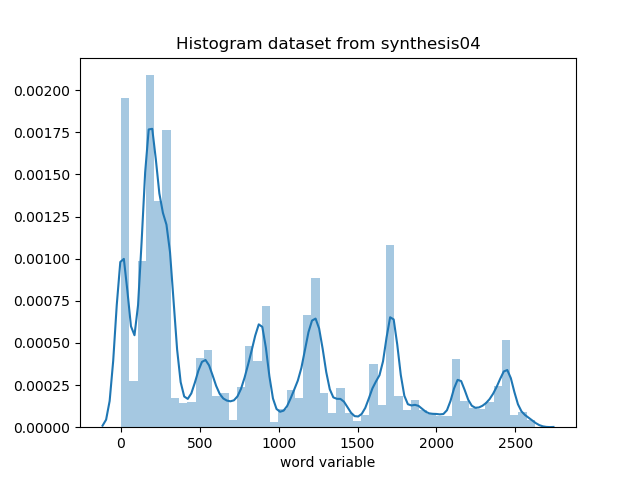
\includegraphics[width=170mm,scale=0.7]{histogramdataset.png}
There are a few words in the dataset with uneven occurrences that cause imbalance in datasets. Here, I have 2 solutions that solve this problem: 
\begin{itemize}
    \item Case 1: I will cut data have count word / max count word < 0.2. 
    \item Case 2: I will generate data from fonts or use a model GAN to generate many word have less distribution to balaced dataset. 
\end{itemize}
Data augmentation is problem need focus in preprocessing. Here, I will recommend a few techniques to handle the data like Smoothing images, scaling, Rotation, background noise. \subsubsection{Data Cleaning}
I have checked file labels.json to check null in target data. And data with null does not exist.
\subsection{Model Deployment}
Based on the work of Shi, Baoguang, Xiang Bai, and Cong Yao. "An end-to-end trainable neural network for image-based sequence recognition and its application to scene text recognition."IEEE transactions on pattern analysis and machine intelligence39.11 (2017): 2298-2304.\cite{crnn}\cite{buildcrnn} \newline
\begin{center}
    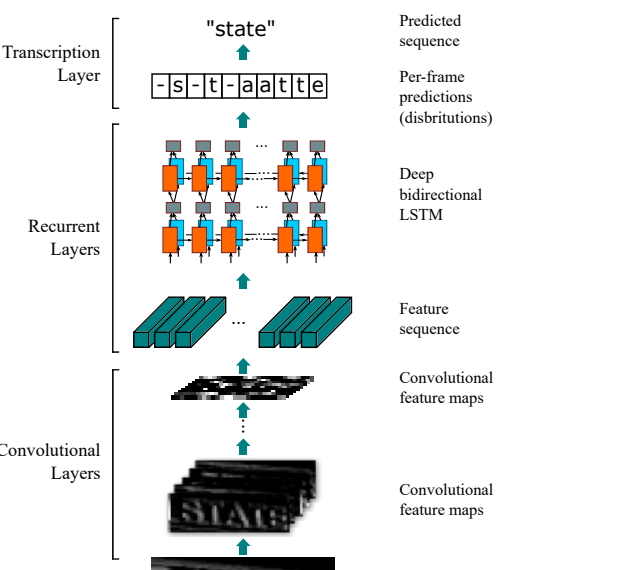
\includegraphics[width=400]{crnn.png}
\end{center}

The architecture consists of three parts from bottom to top: 
\begin{enumerate}
    \item Convolutional layers, which extract a feature sequence from the input image 
    \item Recurrent layers, which predict a label distribution for each frame 
    \item Transcription layer, which translates the per-frame predictions into the final label sequence.\cite{ctc}
\end{enumerate}
Beside model traditional, i will some modifications: 
\begin{enumerate}
    \item Add Dropout, normalization layer to avoid overfitting.
    \item Try some model deep in CNN model(CNN traditional, Lenet, Xception, Resnes)
    \item Add some layers in Recurrent Layers(RNN, GRU, LSTM).
\end{enumerate}
Given the big improbement by attention in machine translation introduced by Luong, et al., 2015)\cite{attention}, i will add attention macharism to CRNN traditional. 
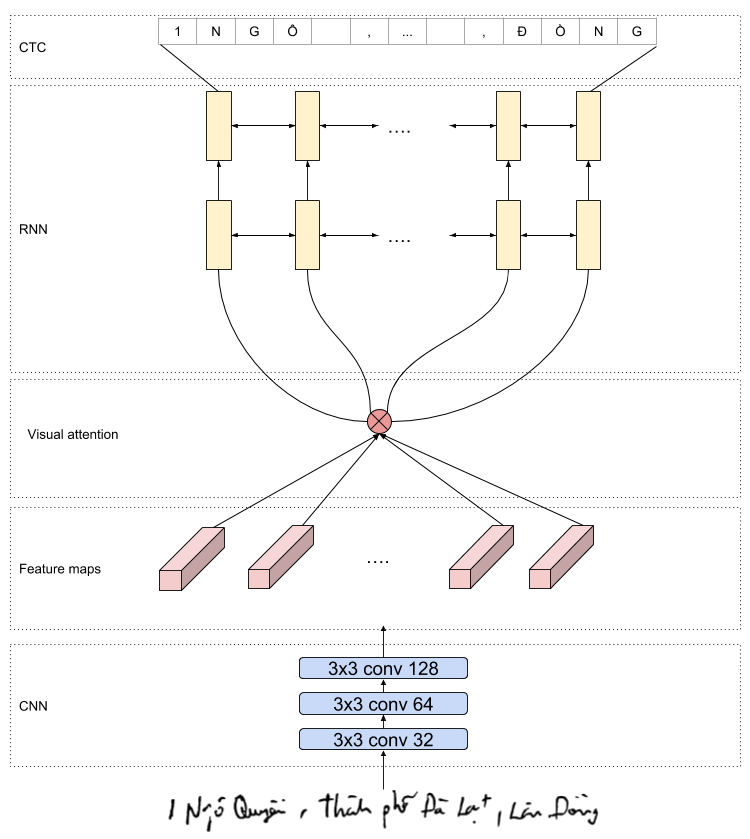
\includegraphics[width=170mm,scale=0.7]{ocr_crnn.png}
\begin{itemize}
    \item The first, we need caculator vector context contain infomation for word current by caculator averaged weight:\newline
    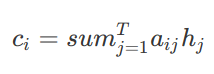
\includegraphics{vector.png}
    \item So How to caculator alpha? Realy, alpha depend infomatioin from h, and also contain infomation of model decoder.\newline
    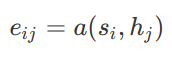
\includegraphics{alpha.png}
    \begin{itemize}
        \item Where alpha is model learning coefficient at each step time. 
    \end{itemize}
    \item Then, normalize total coefficient by use softmax function \newline
    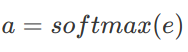
\includegraphics{softmax.png}
    \item Final, we use add vector context for prediction. 
    
\end{itemize}

\subsection{Evaluation}
In printed characters and handwriting recognition, label error rate(also called edit distance error) is the standard metric for evaluation character level classification performance. Give a test set S’ Ç D Dxxz that is independent of S, the label error rate(LER) define by Equation 1:  \newline
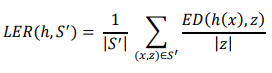
\includegraphics[width=100mm,scale=0.7]{ler.png}
\begin{itemize}
    \item Where h is a temporal classifier as the mean normalized edit distance between its classification; the targets on ��′ ��D(��, ��) is the edit distance between two sequences; �� and �� which is the minimum number of insertions, substitutions, and deletions require to change �� into ��. .This is a natural measure for tasks (such as speech or handwriting recognition) where the aim is to minimize the rate of transcription mistakes. 
    
\end{itemize}
\section{Work Plan(Estimator: 15 days)}
\subsection{Prepare data: 1 days of work}
\begin{itemize}
    \item Get train/validation/test data from our team, preprocessing those data to match with model. 
    \item Perfrom data preprocessing and argumentation, exploration data analysis, data cleaning
\end{itemize}
\subsection{Exploratory data analysis: 3 days of work}
\begin{itemize}
    \item Dealing with Imbalanced data with cut data from a few words appear. After evaluation, I also can generate data with generete from fonts or use model GAN to generate data to balanced data. 
    \item Augmentation data by process Blur, Rotation, Scaling, background noise. 
    \item Clean data with check null in label. 
\end{itemize}
\subsection{ Modeling: 10 days of work}
\begin{itemize}
    \item Deployment the CRNN model and CRNN with attention CRNN in our dataset, tune for high accuracy. 
    \item By the way, try many technical exploratory data analysis to model achieve high results. 
\end{itemize}
\section{Experiments}
\subsection{Datasets}
For all the experiments for scene text recognition, we use the synthetic04 dataset from our company. The dataset contains 4 hundred thousand training images and their corresponding ground truth words.
\subsection{Experiment Details}
The architecture of the convolutional layers is based on the VGG-16 architectures.
We implement the network within the Pytorch framework
\subsubsection{Experiment 1: fixed size, non-fixed size}
\begin{itemize}
    \item Method:  Fixed the size of the image by resizing the image to 32x300. Not fixed image size by resizing image with keep ratio then adding padding to the right of image. 
    \item Evaluation:\newline
    \newline
      \begin{tabular}{|c|c|c|c|c|c|c|c|}
        \hline
        \multicolumn{2}{|>{\columncolor{kugray5}}c|}{}&\multicolumn{4}{c|}{fixed size, non-fixed size}\\
        \multicolumn{2}{|>{\columncolor{kugray5}}c|}{}&\multicolumn{2}{c|}{fixed size} & \multicolumn{2}{c|}{non-fixed size}\\
        \arrayrulecolor{kugray5}
        \arrayrulecolor{black}
        \cline{3-6}
        \multicolumn{2}{|>{\columncolor{kugray5}}c|}{}&by char&by field&by char& by field\\
        \hline
        \multirow{2}{*}{10\% of dataset}
                    & train & 33.5 & 0.0 & 31.4 & 0.0\\
        \cline{2-6}
                    & validation & 26.6 & 0.0 & 21.9 & 0.0\\
        \hline
        \hline
      \end{tabular}
    \item Result:
\end{itemize}

\subsubsection{Experiment 2: Change height}
\begin{itemize}
    \item Method:  I choose the default height of 32, then I increase the height to 64. 
    \item Evaluation:\newline
    \newline
      \begin{tabular}{|c|c|c|c|c|c|c|c|}
        \hline
        \multicolumn{2}{|>{\columncolor{kugray5}}c|}{}&\multicolumn{4}{c|}{fixed size, non-fixed size}\\
        \multicolumn{2}{|>{\columncolor{kugray5}}c|}{}&\multicolumn{2}{c|}{fixed size} & \multicolumn{2}{c|}{non-fixed size}\\
        \arrayrulecolor{kugray5}
        \arrayrulecolor{black}
        \cline{3-6}
        \multicolumn{2}{|>{\columncolor{kugray5}}c|}{}&by char&by field&by char& by field\\
        \hline
        \multirow{2}{*}{10\% of dataset}
                    & train & 33.5 & 0.0 & 31.4 & 0.0\\
        \cline{2-6}
                    & validation & 26.6 & 0.0 & 21.9 & 0.0\\
        \hline
        \hline
      \end{tabular}
    \item Result:
\end{itemize}
\subsubsection{Experiment 3: Learning rate}
\begin{itemize}
    \item Method: I choose the default learning rate of 0.0001, then I increase the learning rate to 0.001.
    \item Evaluation:\newline
    \newline
      \begin{tabular}{|c|c|c|c|c|c|c|c|}
        \hline
        \multicolumn{2}{|>{\columncolor{kugray5}}c|}{}&\multicolumn{4}{c|}{fixed size, non-fixed size}\\
        \multicolumn{2}{|>{\columncolor{kugray5}}c|}{}&\multicolumn{2}{c|}{fixed size} & \multicolumn{2}{c|}{non-fixed size}\\
        \arrayrulecolor{kugray5}
        \arrayrulecolor{black}
        \cline{3-6}
        \multicolumn{2}{|>{\columncolor{kugray5}}c|}{}&by char&by field&by char& by field\\
        \hline
        \multirow{2}{*}{10\% of dataset}
                    & train & 33.5 & 0.0 & 31.4 & 0.0\\
        \cline{2-6}
                    & validation & 26.6 & 0.0 & 21.9 & 0.0\\
        \hline
        \hline
      \end{tabular}
    \item Result:
\end{itemize}
\subsubsection{Experiment 4: Freeze cnn, Freeze rnn}
\begin{itemize}
    \item Method: I will train models with full crnn in 10 epochs. Then, taking the weight of the model to the next 10 epoch, I freeze the crnn or rnn(not train cnn or rnn) in CRNN network. 
    \item Evaluation:\newline
    \newline
      \begin{tabular}{|c|c|c|c|c|c|c|c|}
        \hline
        \multicolumn{2}{|>{\columncolor{kugray5}}c|}{}&\multicolumn{4}{c|}{fixed size, non-fixed size}\\
        \multicolumn{2}{|>{\columncolor{kugray5}}c|}{}&\multicolumn{2}{c|}{fixed size} & \multicolumn{2}{c|}{non-fixed size}\\
        \arrayrulecolor{kugray5}
        \arrayrulecolor{black}
        \cline{3-6}
        \multicolumn{2}{|>{\columncolor{kugray5}}c|}{}&by char&by field&by char& by field\\
        \hline
        \multirow{2}{*}{10\% of dataset}
                    & train & 33.5 & 0.0 & 31.4 & 0.0\\
        \cline{2-6}
                    & validation & 26.6 & 0.0 & 21.9 & 0.0\\
        \hline
        \hline
      \end{tabular}
    \item Result:
\end{itemize}
\subsubsection{Experiment 5: Add attention}

\subsubsection{Experiment 6: Remove rnn only train cnn by densenet121 + CTC Loss}
\begin{itemize}
    \item Method: I use model Densenet + CTC Loss. Detail at here:
    \newline
    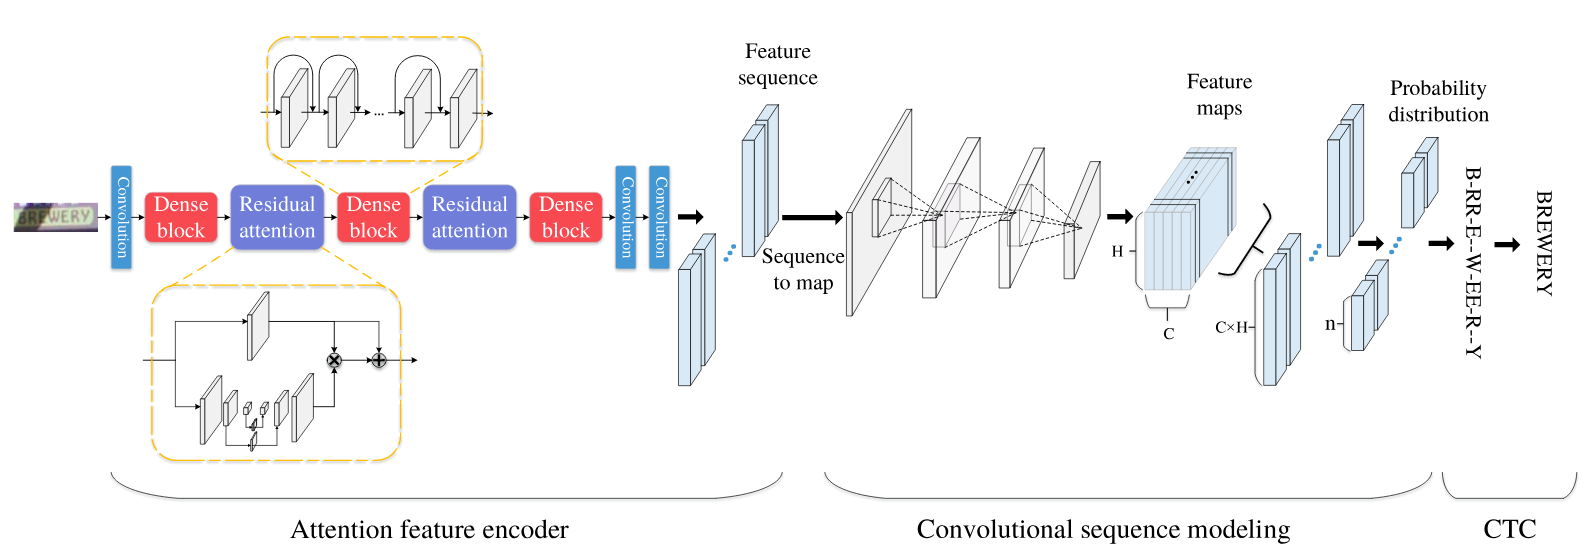
\includegraphics[width=160mm]{densenet_ctc.png}
    \item Evaluation:\newline
     \newline
        \begin{tabular}{|c|c|c|c|}
            \hline
            \multicolumn{2}{|>{\columncolor{kugray5}}c|}{}&\multicolumn{2}{c|}{Densenet+ CTC}\\
            \arrayrulecolor{kugray5}
            \arrayrulecolor{black}
            \cline{3-4}
            \multicolumn{2}{|>{\columncolor{kugray5}}c|}{}&by char&by field\\
            \hline
            \multirow{2}{*}{full of dataset}
                        & train & 97.97 & 86.06\\
            \cline{2-4}
                        & validation & 87.26 & 64.72\\
            \hline
            \hline
        \end{tabular}
    \item Result:
\end{itemize}
\subsubsection{Experiment 7: Shuffle and non Shuffle}
\begin{itemize}
    \item Method: The first, sort all line images in training set based on the length of label text. Next, training with three methods: 
    \item Evaluation:
    \begin{enumerate}
        \item Do not shuffle the training set
        \newline
        \begin{tabular}{|c|c|c|c|}
            \hline
            \multicolumn{2}{|>{\columncolor{kugray5}}c|}{}&\multicolumn{2}{c|}{not shuffle}\\
            \arrayrulecolor{kugray5}
            \arrayrulecolor{black}
            \cline{3-4}
            \multicolumn{2}{|>{\columncolor{kugray5}}c|}{}&by char&by field\\
            \hline
            \multirow{2}{*}{10\% of dataset}
                        & train & 33.5 & 0.0\\
            \cline{2-4}
                        & validation & 26.6 & 0.0\\
            \hline
            \hline
        \end{tabular}
        \item Shuffle the training set after 2 epoch
        \newline
        \begin{tabular}{|c|c|c|c|}
            \hline
            \multicolumn{2}{|>{\columncolor{kugray5}}c|}{}&\multicolumn{2}{c|}{shuffle after 2 epoch}\\
            \arrayrulecolor{kugray5}
            \arrayrulecolor{black}
            \cline{3-4}
            \multicolumn{2}{|>{\columncolor{kugray5}}c|}{}&by char&by field\\
            \hline
            \multirow{2}{*}{10\% of dataset}
                        & train & 33.5 & 0.0\\
            \cline{2-4}
                        & validation & 26.6 & 0.0\\
            \hline
            \hline
        \end{tabular}
        \item Shuffle at the beginning of training process
                \newline
        \begin{tabular}{|c|c|c|c|}
            \hline
            \multicolumn{2}{|>{\columncolor{kugray5}}c|}{}&\multicolumn{2}{c|}{shuffle}\\
            \arrayrulecolor{kugray5}
            \arrayrulecolor{black}
            \cline{3-4}
            \multicolumn{2}{|>{\columncolor{kugray5}}c|}{}&by char&by field\\
            \hline
            \multirow{2}{*}{10\% of dataset}
                        & train & 33.5 & 0.0\\
            \cline{2-4}
                        & validation & 26.6 & 0.0\\
            \hline
            \hline
        \end{tabular}
    \end{enumerate}
    \item Result:
\end{itemize}
\subsubsection{Experiment 8: Train full dataset}

\subsection{Comparative Evaluation}

\section{Future Plan}
I have focus to model encoder and decoder by openmnt development. It is model to prediction image to text take care math in latex. The architecture show: \newline
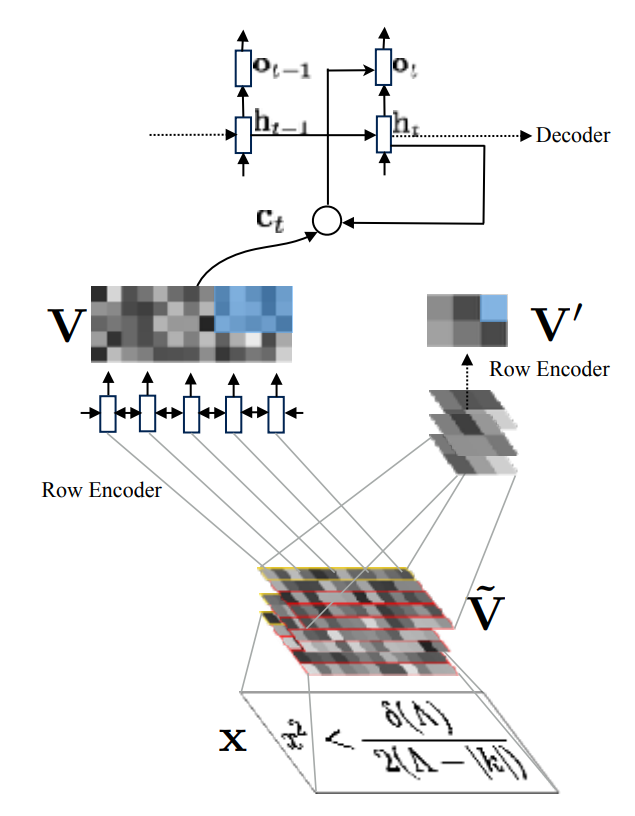
\includegraphics[width=170mm,scale=0.7]{openmnt.png}
The model first extracts image features using a convolution neural network(CNN) and arranges the features in a grid. Each row is then encoded using a recurrent neural network(RNN). These encoded using a recurrent neural network(RNN). These encoded features are then used by an RNN decoder with a visual attention mechanism. The decoder implements a conditional language model over the vocabulary, and the whole model is trained to maximize the likelihood of the observed markup. \cite{openmnt}


\bibliographystyle{unsrt}
\bibliography{sample}
\end{document}
